\documentclass{article}
\usepackage[english]{babel}
\usepackage{geometry,amsmath,amssymb,graphicx}
\geometry{a4paper}

%%%%%%%%%% Start TeXmacs macros
\newcommand{\tmaffiliation}[1]{\\ #1}
\newcommand{\tmop}[1]{\ensuremath{\operatorname{#1}}}
\newcommand{\tmtextit}[1]{\text{{\itshape{#1}}}}
%%%%%%%%%% End TeXmacs macros

\begin{document}

\title{Machine learning}

\author{
  Youjun Hu
  \tmaffiliation{yjhu@ipp.cas.cn}
}

\maketitle

\

\section{Introduction}

Artificial intelligence (AI) research has tried many different approaches
since its founding. In the first decades of the 21st century, the AI research
is dominated by highly mathematical statistical machine learning (ML), which
has proved highly successful, helping to solve many challenging problems in
real life.

Many problems in AI can be solved theoretically by searching through many
possible solutions: Reasoning can be reduced to performing a search. Simple
exhaustive searches are rarely sufficient for most real-world problems. The
solution, for many problems, is to use "heuristics" or "rules of thumb" that
prioritize choices in favor of those more likely to reach a goal. A very
different kind of search came to prominence in the 1990s, based on the
mathematical theory of optimization. Modern machine learning is based on these
methods. Instead, of using detailed explanations to guide the search, it uses
a combination of{\cite{nielsen2015neural}}: (a) general architectures; (b)
trying trillions of possibilities, guided by simple ideas (like gradient
descent) for improvement; and (c) the ability to recognize progress.

I am interested in applying machine learning to problems in computational
physics problems that traditional numerical methods can not easily handle
either because of its computational costs being too high or its traditional
algorithms are too complicated to easily implement.

Enrico Fermi once criticized the complexity of a model (that contains many
free parameters) by quoting Johnny von Neumann ``With four parameters I can
fit an elephant, and with five I can make him wiggle his trunk''.

What Fermi implies is that it is easy to fit existing data and what is
important is to have a model with predicting capability (fitting data not seen
yet). The artificial neural network method tackles this difficulty by
increasing the number of free parameters to millions, with the hope of
obtaining predicting capability.

\section{Neural network}

Neural networks consists of multiple layers of interconnected nodes (neurons),
each having a weight for a connection, a bias and activation function. Each
layer build upon the previous layer. This progression of computations through
the network is called forward propagation. Another process called
backpropagation uses algorithms which moves backwards through the layers to
efficiently compute the partial derivatives of the loss function with respect
to the weights and biases. Combining the forward and backward propagation, we
can calculate errors in predictions and then adjusts the weights and biases
using the gradient descent method. This process is called training.

\subsection{ Node (neuron or unit), weight, bias, and activation}

As is shown in Fig. \ref{22-3-13-a1}, we use $w_{j k}^l$ to denote the weight
for the connection from the $k^{\tmop{th}}$ neuron in the $(l -
1)^{\tmop{th}}$ layer to the $j^{\tmop{th}}$ neuron in the $l^{\tmop{th}}$
layer. Use $b_j^l$ to denote the bias of the $j^{\tmop{th}}$ neuron in the
$l^{\tmop{th}}$ layer.

\begin{figure}[h]
  \raisebox{-0.369502148506993\height}{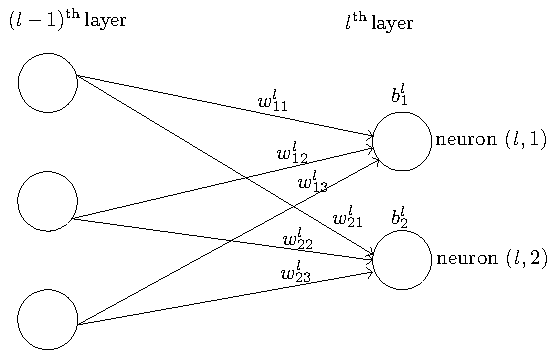
\includegraphics[width=9.35164961301325cm,height=5.99124360487997cm]{machine_learning-1.pdf}}
  \caption{\label{22-3-13-a1}Definition of layers, neurons, weights, and
  biases in a neural network. The $j^{\tmop{th}}$ neuron in the
  $l^{\tmop{th}}$ layer is referred to as neuron $(l, j)$}
\end{figure}

\

We use $a_j^l$ to denote the output (activation) of the $j^{\tmop{th}}$
neuron in $l^{\tmop{th}}$ layer. A neural network model assumes that $a_j^l$
is related to the $a^{l - 1}$ (output of the previous layer) via
\begin{equation}
  \label{22-3-9-e2} a^l_j = \sigma \left( \sum_k w_{j k}^l a^{l - 1}_k + b^l_j
  \right),
\end{equation}
where the summation is over all neurons in the $(l - 1)^{\tmop{th}}$ layer and
$\sigma$ is a function called activation function which can take various
forms, e.g., step function,
\begin{equation}
  \sigma (z) = \left\{ \begin{array}{l}
    1 \tmop{if} z \geqslant 0\\
    0 \quad \tmop{else}
  \end{array} \right.,
\end{equation}
rectified linear unit (ReLU),
\begin{equation}
  \sigma (z) = \max (0, z),
\end{equation}
and sigmoid function (``S''-shaped curve, also called logistic function)
\begin{equation}
  \sigma (z) = \frac{1}{1 + \exp (- z)} .
\end{equation}
Define $z_j^l$ by
\begin{equation}
  \label{22-3-9-1} z^l_j = \sum_k w_{j k}^l a^{l - 1}_k + b^l_j,
\end{equation}
which can be interpreted as an weighted input to the neuron $(l, j)$, then Eq.
(\ref{22-3-9-e2}) is written as
\begin{equation}
  a_j^l = \sigma (z^l_j) .
\end{equation}
In matrix form, Eq. (\ref{22-3-9-1}) is written as
\begin{equation}
  z^l = w^l a^{l - 1} + b^l,
\end{equation}
where $w^l$ is a $J \times K$ matrix, $z^l$ \ and $b^l$ are column vectors of
length $J$, $a^{l - 1}$ is a column vector of length $K$, where $J$ and $K$
are the number of neurons in the $l^{\tmop{th}}$ layer and $(l -
1)^{\tmop{th}}$ layer, respectively.

The input layer is where data inputs are provided, and the output layer is
where the final prediction is made. The input and output layers of a deep
neural network are called visible layers. The layers between the input layer
and output layer are called hidden layers. Note that the input layer is
usually not considered as a layer of the network since it does not involve any
computation. In tensorflow, layers refer to the computing layers (i.e., hidden
layers and the output layer, not including the input layer). The activation
function of each layer can be different. The activation function of the output
layer is often chosen as None, ReLU, logistic/tanh, and is usually different
from those used in the hidden layers. Here ``None'' means activation $\sigma
(z) = z$.

\subsection{Loss function}

Define a loss (cost, error) function by
\begin{equation}
  \label{22-3-9-e1} C (w, b) \equiv \frac{1}{2 n} \sum_x \| y (x) - a^L \|^2,
\end{equation}
where $w$ and $b$ denotes the collection of all weights and biases in the
network, $n$ is the total number of training examples $x$, the summation is
over all the training examples, $y (x)$ is the desired output from the network
(i.e., correct answer) when $x$ is the input, and $a^L$ is the actual output
from the output layer of the network and is a function of $w, b$, and $x$.
Note that $y$ and $a^L$ are vectors (with number of elements being the number
of neurons in the output layer) and $\| \ldots \|$ denotes the vector norm.
Explicitly writing out the vector norm, Eq. (\ref{22-3-9-e1}) is written as
\begin{equation}
  \label{22-3-9-e1m} C (w, b) \equiv \frac{1}{2 n} \sum_x \sum^{N_L}_{j = 1}
  (y_j (x) - a^L_j)^2,
\end{equation}
where $N_L$ is the number of neurons in the output layer.

The cost function is the average error of the approximate solution away from
the desired exact solution. So the goal of a learning algorithm is to find
weights and biases that minimize the cost function. To minimize the cost
function over $(w, b)$ using the gradient descent method, we need to compute
the partial derivatives $\partial C / \partial w^l_{j k}$ and $\partial C /
\partial b^l_j$. Next we will discuss how to compute them.

\subsection{Gradients of loss function}

Note that the loss function involves an average over all the training
examples. Denote the loss function for a specific training example by $C_x$,
i.e.,
\begin{equation}
  \label{22-3-11-a6} C_x = \frac{1}{2} \sum^{N_L}_{j = 1} (y_j (x) - a^L_j)^2,
\end{equation}
then expression (\ref{22-3-9-e1m}) is written as
\begin{equation}
  C = \frac{1}{n} \sum_x C_x,
\end{equation}
Then the partial derivatives $\partial C / \partial w^l_{j k}$ and $\partial C
/ \partial b^l_j$ can be written as the sum of $\partial C_x / \partial w^l_{j
k}$ and $\partial C_x / \partial b^l_j$, i.e.,
\begin{equation}
  \label{22-3-11-a3} \frac{\partial C}{\partial w_{j k}^l} = \frac{1}{n}
  \sum_x \frac{\partial C_x}{\partial w_{j k}^l},
\end{equation}

\begin{equation}
  \label{22-3-11-a4} \frac{\partial C}{\partial b_j^l} = \frac{1}{n} \sum_x
  \frac{\partial C_x}{\partial b_j^l} .
\end{equation}
The above formulas indicate that, once $\partial C_x / \partial w^l_{j k}$ and
$\partial C_x / \partial b^l_j$ are known, obtaining \ $\partial C / \partial
w^l_{j k}$ and $\partial C / \partial b^l_j$ is trivial, i.e., just averaging
them. Therefore, we will focus on $C_x$ (i.e., the cost function for a fixed
training example) and discuss how to compute $\partial C_x / \partial w^l_{j
k}$ and $\partial C_x / \partial b^l_j$.

In practice, we do not sum over all the training examples. Instead, we
average the derivative over a small number (say 16) of training examples (a
mini batch) and use these approximate derivatives to advance a step. For the
next step, we stochastically change to using a different mini batch. This is
called stochastic gradient descent (SGD) method.

\subsection{Back-propagating algorithm}

The cost function $C_x$ is a function of weights and biases of all neurons
(the input $x$ and output $y (x)$ are fixed parameters). For a specific neuron
$(l, j)$, its weights and biases enter $C_x$ via the combination $z_j^l =
\sum_k w_{j k}^l a^{l - 1}_k + b^l_j$. Then it is useful to define the
following partial derivative:
\begin{equation}
  \label{22-3-11-p1} \delta^l_j \equiv \frac{\partial C_x}{\partial z_j^l},
\end{equation}
where the partial derivative are taken with fixed weights and biases for all
neurons except neuron $(l, j)$. Note that the $a_k^{l - 1}$ appearing in the
expression of $z_j^l$ does not depend on $w^l_{j k}$ or $b^l_j$. It only
depends on the weights and biases in the layers $\leqslant (l - 1)$, which are
all fixed when taking the derivative in expression (\ref{22-3-11-p1}).
$\delta^l_j$ defined in expression (\ref{22-3-11-p1}) is often called the
error of neuron $(l, j)$.

Using the chain rule, \ $\partial C_x / \partial w^l_{j k}$ and $\partial C_x
/ \partial b^l_j$ can be expressed in terms of $\delta^l_j$:
\begin{equation}
  \frac{\partial C_x}{\partial b_j^l} = \frac{\partial C_x}{\partial z_j^l} 
  \frac{\partial z^l_j}{\partial b_j^l} = \delta^l_j,
\end{equation}
and
\begin{equation}
  \frac{\partial C_x}{\partial w_{j k}^l} = \frac{\partial C_x}{\partial
  z_j^l}  \frac{\partial z^l_j}{\partial w_{j k}^l} = \delta^l_j a_k^{l - 1} .
\end{equation}
Therefore, if $\delta^l_j$ is known, it is trivial to compute the gradients
needed in the gradient descent method.



\

\raisebox{-0.369502148506993\height}{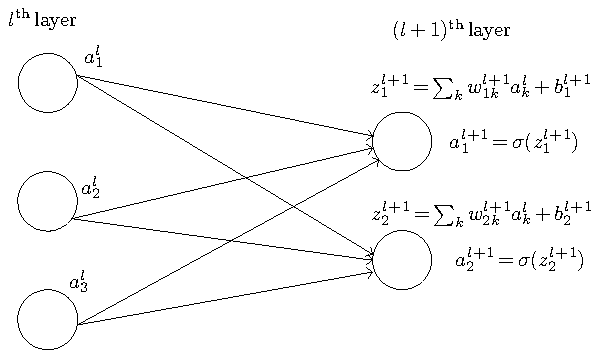
\includegraphics[width=10.0733799029254cm,height=5.99124360487997cm]{machine_learning-2.pdf}}

\

\

\

For the output layer ($L^{\tmop{th}}$ layer), $\delta^l_j$ defined in Eq.
(\ref{22-3-11-p1}) is written as
\begin{equation}
  \delta^L_j = \frac{\partial C_x}{\partial z_j^L} = \frac{\partial
  C_x}{\partial a^L_j}  \frac{\partial a^L_j}{\partial z_j^L} .
\end{equation}
The dependence of $C_x$ on $a_j^L$ is explicitly given by Eq.
(\ref{22-3-11-a6}), from which the above expression for $\delta_j^L$ is
written as
\begin{equation}
  \delta^L_j = (a^L_j - y_j (x)) \sigma' (z_j^L) .
\end{equation}
Therefore $\delta^L_j$ is easy to compute.

Backpropagation is a way of computing $\delta^l_j$ for every layer using
recurrence relations: the relation between $\delta^l$ and $\delta^{l + 1}$.
Noting how the error is propagating through the network, we know the following
identity:
\begin{equation}
  \frac{\partial C_x}{\partial z_J^l} d z^l_J = \sum_j \frac{\partial
  C_x}{\partial z_j^{l + 1}} d z^{l + 1}_j,
\end{equation}
with
\begin{equation}
  d z_j^{l + 1} = w^{l + 1}_{j J} d (a^l_J),
\end{equation}
i.e.,
\begin{equation}
  d z_j^{l + 1} = w^{l + 1}_{j J} \sigma' (z^l_J) d z^l_J .
\end{equation}
Therefore
\begin{equation}
  \frac{\partial C_x}{\partial z_J^l} = \sum_j \frac{\partial C_x}{\partial
  z_j^{l + 1}} w^{l + 1}_{j J} \sigma' (z^l_J) .
\end{equation}
i.e.,
\begin{equation}
  \label{22-3-14-a1} \delta^l_J = \sum_j \delta^{l + 1}_j w^{l + 1}_{j J}
  \sigma' (z^l_J) .
\end{equation}
Equation (\ref{22-3-14-a1}) gives the recurrence relations of computing
$\delta^l$ from $\delta^{l + 1}$. This is called the backpropagation
algorithm. Eq. (\ref{22-3-14-a1}) can be written in the matrix form:
\begin{equation}
  \delta^l = ((w^{l + 1})^T \delta^{l + 1}) \odot \sigma' (z^l),
\end{equation}
where $T$ stands for matrix transpose, $\odot$ is the element-wise product.

\begin{thebibliography}{1}
  \bibitem[1]{nielsen2015neural}Michael~A Nielsen. {\newblock}\tmtextit{Neural
  networks and deep learning},  volume~25. {\newblock}Determination Press:
  http://neuralnetworksanddeeplearning.com/, 2015.{\newblock}
\end{thebibliography}

\section{miscs}

\

\end{document}
